
Mesa3D一开始实现绘制渲染管线是通过纯软件计算实现的,也就是全都是在CPU端计算实现的,这种实现方法就是图\ref{fig:Mesa3D}里面的swrast模块,而现在大部分平台包括龙芯平台都采用CPU+GPU这种硬件加速的方式来实现整个渲染过程,该流程主要如图\ref{fig:Mesa3D-Flow}所示:

\begin{figure}[H] 
  \centering
  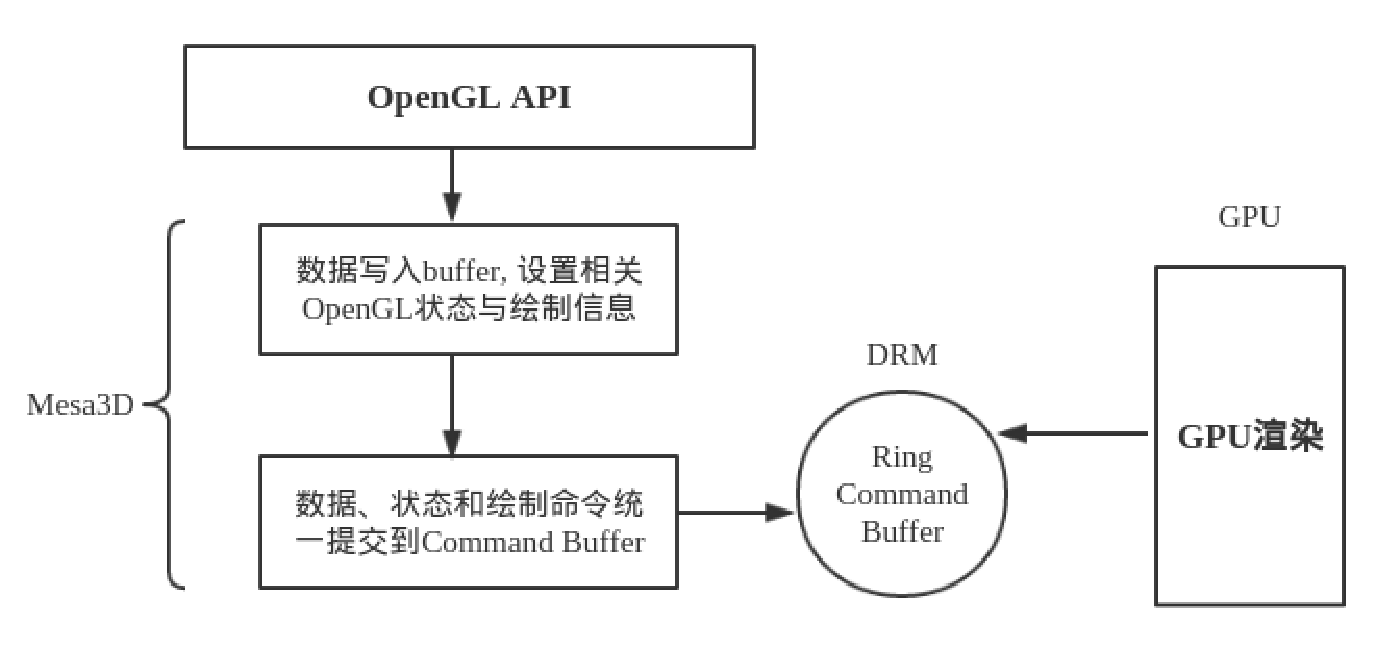
\includegraphics[width=10cm,height=7cm]{figures/chap02/Mesa3D-Flow}
  \caption{Mesa3D的硬件加速实现}
  \label{fig:Mesa3D-Flow}
\end{figure}

在这个过程中Mesa3D负责解析OpenGL的绘制命令块,然后把相关顶点数据、纹理数据、属性数据等存入到对应缓存区中,然后通过Gallium3D的相关接口准备好数据存放信息、绘制命令、状态信息等命令包,然后调用libdrm库将这些命令包写入到Ring Command Buffer,接着通知GPU来读取命令数据,开始GPU的图形渲染流程。


